\documentclass[]{article}
\usepackage{polski}
\usepackage[utf8]{inputenc}
\usepackage{mathtools}
\usepackage{pgfplots}
\usepackage{listings}
\usepackage{enumitem}
\usepackage{mathtools}

%opening
\title{\textbf{ Metody Numeryczne 2\\Laboratorium 2\\}
Interpolacja funkcjami sklejanymi liniowymi z~przestrzeni $S_1(\Delta_n, 0)$}
\author{Szymon Adach}

\begin{document}

\maketitle


\section{Treść zadania}

Zadanie 6: Interpolacja funkcjami sklejanymi liniowymi z przestrzeni $S_1(\Delta_n, 0)$. Zagęszczanie podziału $\Delta_n$ aż do osiągnięcia błędu rzeczywistego, mierzonego w środkach posprzedziałów, mniejszego od $\varepsilon$.	
\section{Opis metody}
Niech $\Delta_n$ będzie podziałem odcinka $[a,b]$:
\[ \Delta_n : a = x_0 < x_1 < \dots < x_n = b \]
Wówczas definiujemy przestrzeń funkcji:
\[ S_m(\Delta_n, k) = \{ s \in C^k([a,b]) : s |_{[x_{i-1}, x_i]} \in P_m([x_{i-1},x_i]), \quad i = 1,\dots,m \} \]
gdzie $P_m$ to przestrzeń wielomianów stopnia $m$. 
W tych funkcjach sklejanych funkcją bazową jest funkcja:
\[ \psi(x) = \begin{cases}
x + 1 & \text{dla } x \in [-1, 0] \\
1 - x & \text{dla } x \in [0, 1] \\
0 & \text{dla pozostałych } x
\end{cases} \]

Definiujemy również funkcję opartą na węzłach $x_{i-1}, x_i, x_{i+1}$, $i = 0,1,\dots,n$:
\[ \psi_i(x) = \psi \left( \frac{x-x_i}{h} \right), \qquad i = 0,1,\dots,n \]
dzięki której możemy zdefiniować wielomian sklejany
\[ s(x) = \sum_{j=0}^n a_j \psi_j(x) \]

Zadanie można podzielić na następujące podproblemy:
\begin{enumerate}
	\item \textbf{Podział odcinka na n części i znalezienie splajnów.}
	\begin{lstlisting}[mathescape, language=Matlab]
	// f - funkcja interpolowana
	x = linspace(a, b, n+1);
	h = (b-a)/n;
	val = zeros(1, length(x)-1);
	for k=1:length(x)-1
	  mid = (x(k) + h/2);
	  val(k) = f(x(k)) * (x(k+1) - mid)/ ...
	  (x(k+1)-x(k)) + f(x(k+1)) * ...
	  (mid - x(k))/(x(k+1) - x(k));     
	end
	\end{lstlisting}
	\item \textbf{Sprawdzenie wartości błędu maksymalnego (mierzonego w środkach podprzedziałów)}
	\\*
	Zgodnie z poleceniem dokonywane jest obliczenie błędu maksymalnego i~porównanie jego wartości z $\varepsilon$ podanym przez użytkownika. Jeżeli interpolacja nie spełnia zadanego warunku, to program przechodzi do pierwszego kroku przy dwukrotnym zagęszczeniu podziału $\Delta_n$. W przeciwnym przypadku program przechodzi do punktu trzeciego.
	\begin{lstlisting}[mathescape, language=Matlab]
	val_diff = zeros(1, length(val));
	for k=1:length(x)-1
	  mid = (x(k) + h/2);
	  val_diff(k) = abs(f(mid) - val(k));
	end
	max_err = max(val_diff);
	\end{lstlisting}
	\item \textbf{Narysowanie wykresów funkcji interpolowanej i splajnów.}
\end{enumerate}
\section{Działanie programu}
Program został napisany w MATLAB-ie, składa się z 4 plików:
\begin{itemize}
	\item \textbf{spline.m} - pętla główna programu
	\item \textbf{calc\_mid.m} - obliczanie splajnów
	\item \textbf{err.m} - obliczenie błędu maksymalnego
	\item \textbf{plotter.m} - rysowanie wykresów
\end{itemize}
Program jest uruchamiany poleceniem \textbf{find\_zeroes(a, b, n, e, f)}, gdzie:
\begin{itemize}
	\item \textbf{a, b} - początek i koniec przedziału, na którym interpolujemy
	\item \textbf{n} - liczba podprzedziałów
	\item \textbf{e} - oczekiwana dokładność
	\item \textbf{f} - funkcja interpolowana (w MATLAB-ie uchwyt do funkcji)
\end{itemize}
Po wykonaniu obliczeń prezentowany jest wykres funkcji interpolowanej oraz splajnów, a w konsoli wypisywana jest wynikowa liczba podprzedziałów i uzyskana dokładność.
\section{Przykłady}
\begin{enumerate}

\item \textbf{Wywołanie:} \verb|spline(0.01, 0.5, 20, 0.01, @(x)sin(1./x))|
\\\textbf{Wyjście:}
\\Liczba wezlow: 20480
\\Blad maksymalny (liczony w srodkach): 0.006842
\begin{center}
	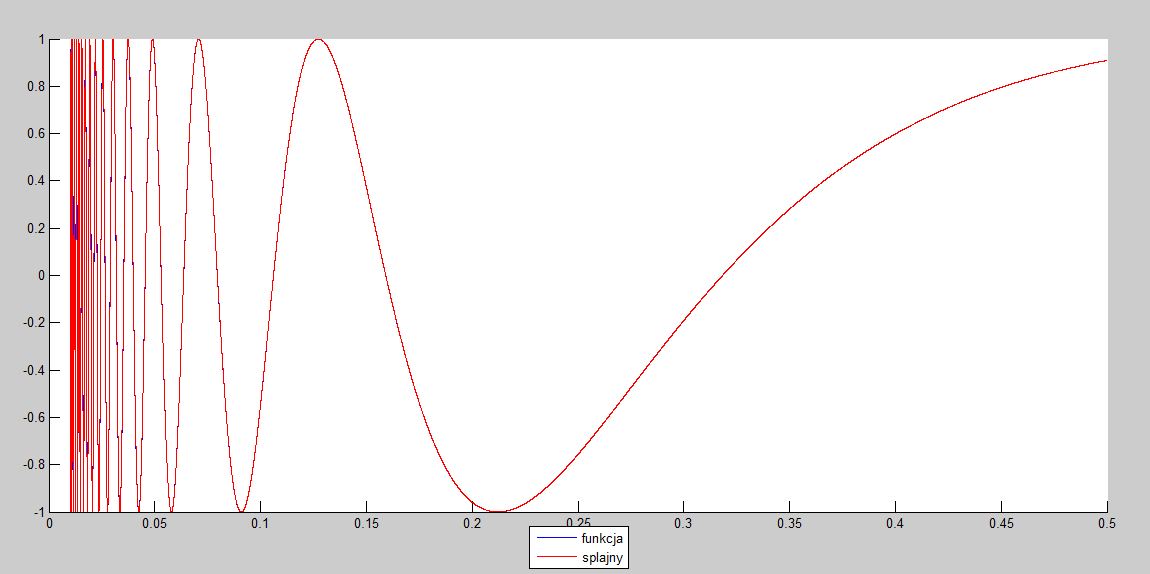
\includegraphics[scale = 0.4]{1.png}
\end{center}
Komentarz: Przy zadanej dużej dokładności i  czas działania funkcji jest zwiększony ze względu na "gęstość" wykresu funkcji, która wpływa na liczbę operacji.
\newpage
\item \textbf{Wywołanie:} \verb|spline(0.01, 0.5, 4, 0.25, @(x)sin(1./x))|
\\\textbf{Wyjście:}
\\Liczba wezlow: 4096
\\Blad maksymalny (liczony w srodkach): 0.154378
\begin{center}
	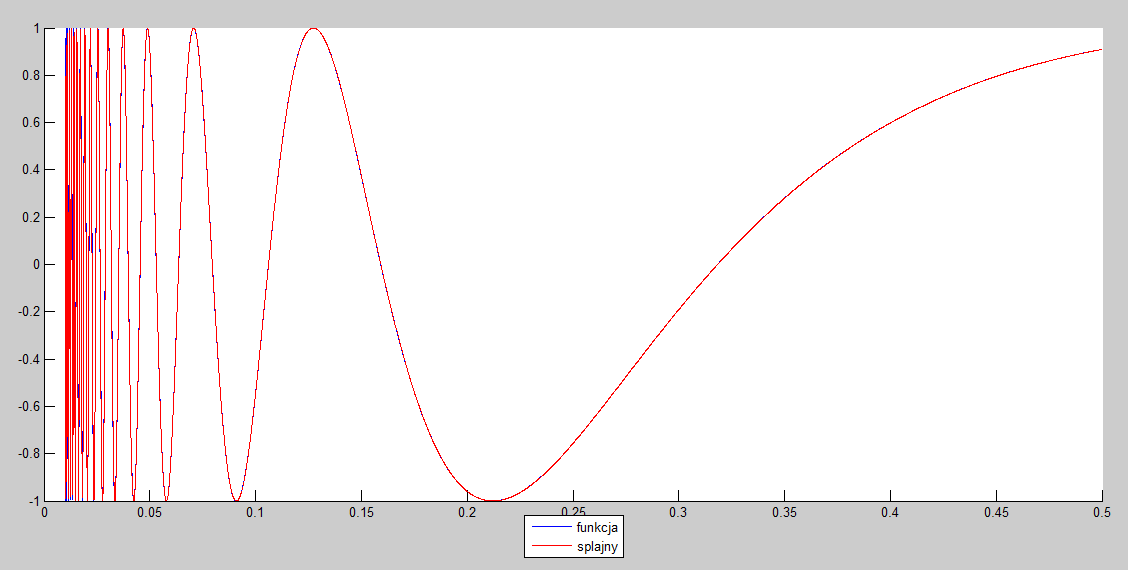
\includegraphics[scale = 0.4]{2.png}
\end{center}

\item \textbf{Wywołanie:} \verb|spline(0, 50, 8, 0.25, @(x)sin(x))|
\\\textbf{Wyjście:}
\\Liczba wezlow: 64
\\Blad maksymalny (liczony w srodkach): 0.074659
\begin{center}
	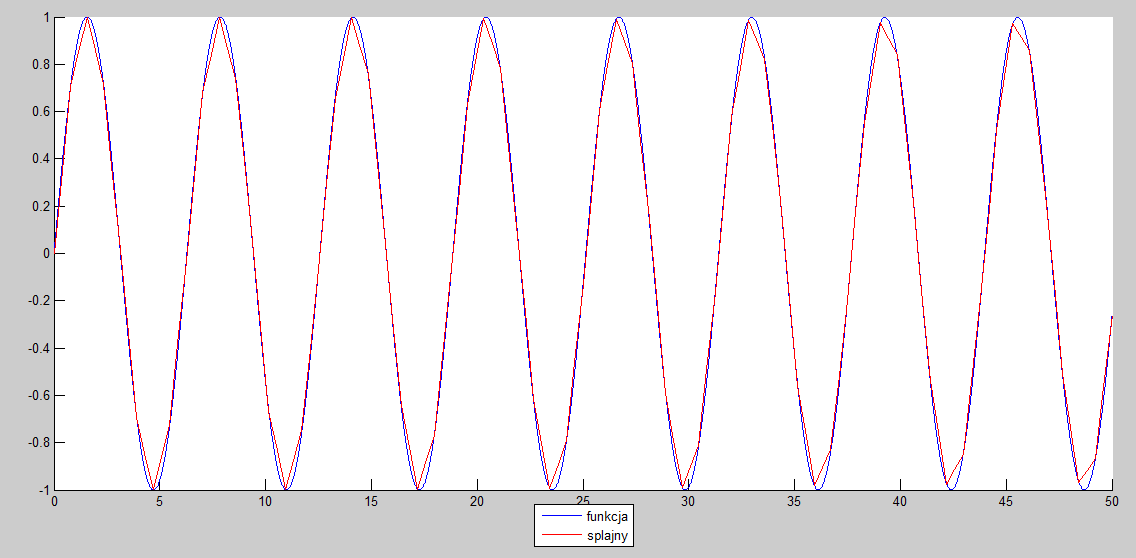
\includegraphics[scale = 0.4]{3.png}
\end{center}
\newpage
\item \textbf{Wywołanie:} \verb|spline(0, 25, 2, 3, @(x)x.^2.-21.*x+104)|
\\\textbf{Wyjście:}
\\Liczba wezlow: 8
\\Blad maksymalny (liczony w srodkach): 2.441406
\begin{center}
	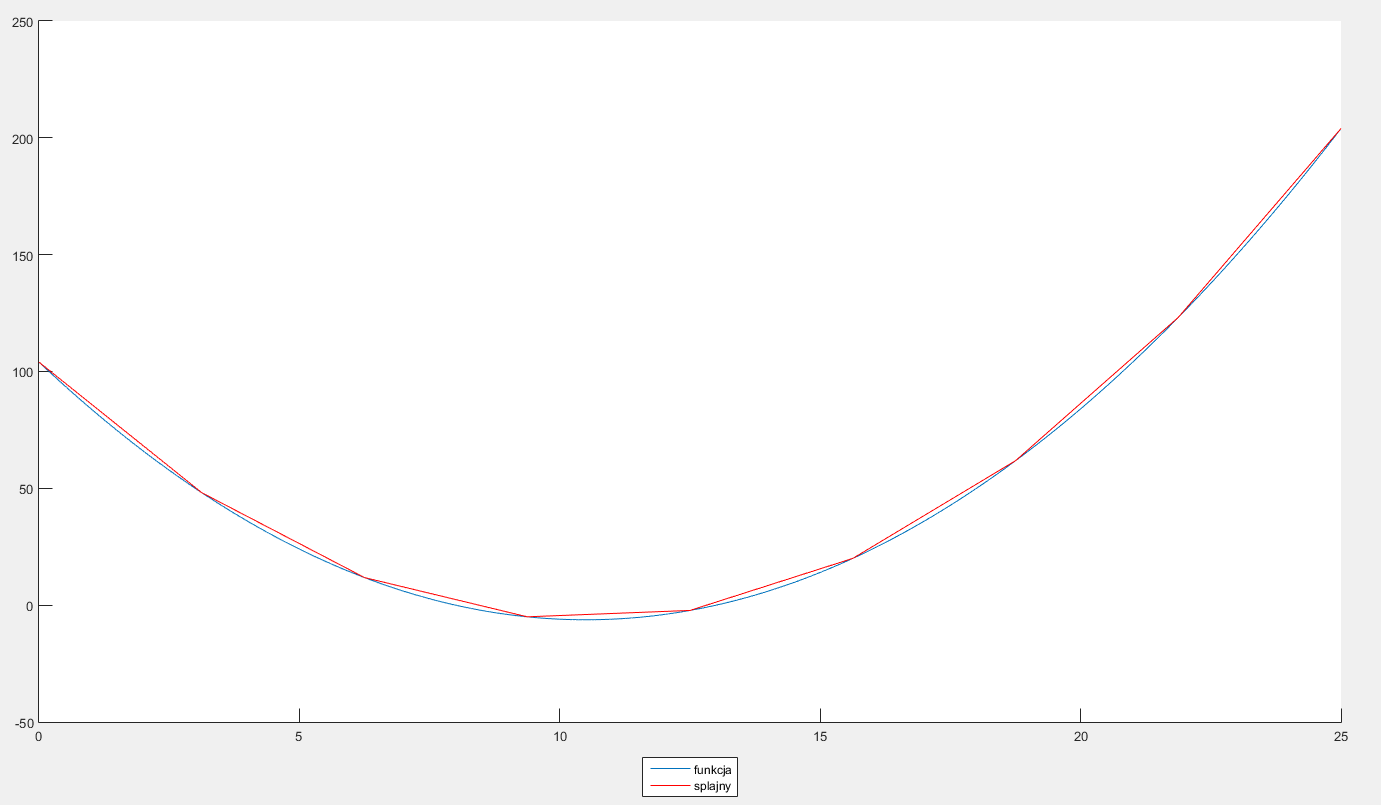
\includegraphics[scale = 0.33]{4.png}
\end{center}
\end{enumerate}
\end{document}
